\section{Results}
Results from the logistic regression are included in figures 
\ref{fig:logistic1}, \ref{fig:logistic2}, \ref{fig:logistic3}, 
\ref{fig:logistic-roc}.


\section{Results}\label{fig:logistic1}
\begin{figure}[H]
\begin{center}
    \subfloat[]{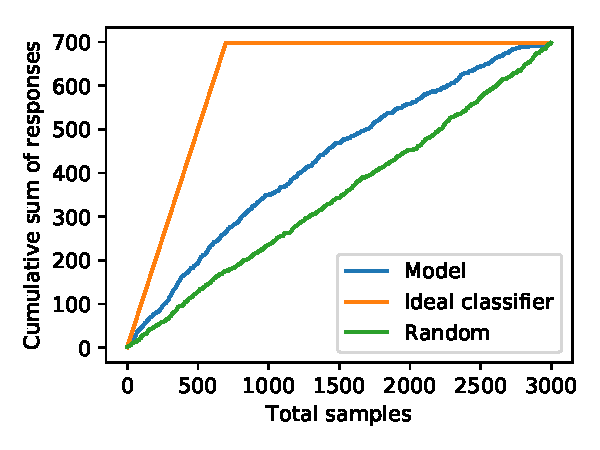
\includegraphics[width=0.4\textwidth, height=0.25\textheight]{figures/logistic_none_cumul}} 
    \subfloat[]{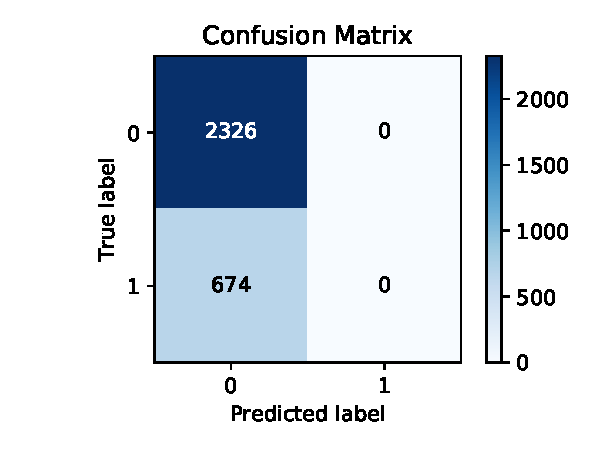
\includegraphics[width=0.4\textwidth, height=0.25\textheight]{figures/logistic_none_confmat}} \\
    \subfloat[]{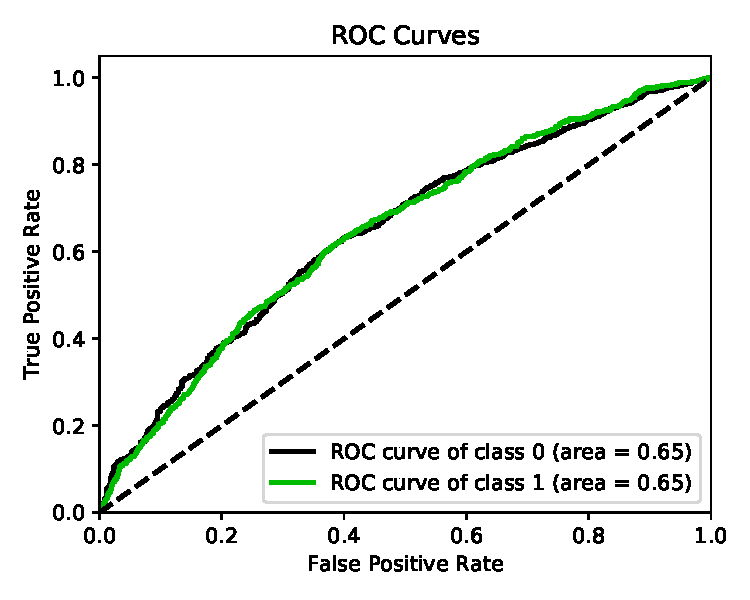
\includegraphics[width=0.5\textwidth]{figures/logistic_none_roc}}
\end{center}
\caption[caption]{Performance analysis for basic logistic regression.}
\end{figure}
\begin{figure}[H]
\begin{center}
    \subfloat[Random oversampling]{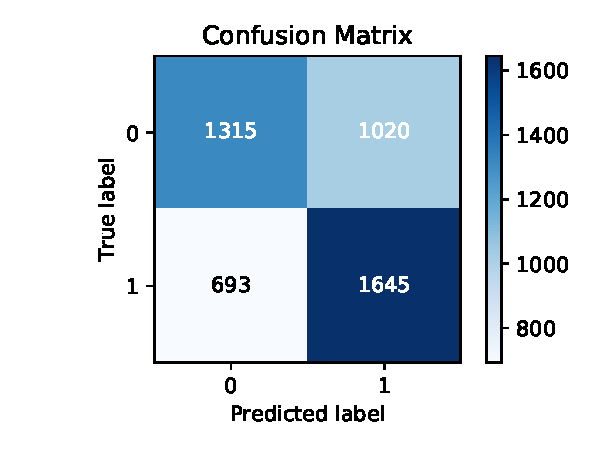
\includegraphics[width=0.4\textwidth, height=0.25\textheight]{figures/logistic_random_oversampling_confmat}} 
    \subfloat[ADASYN]{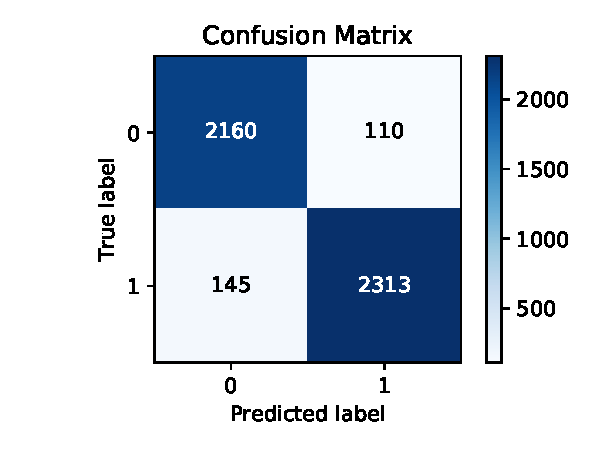
\includegraphics[width=0.4\textwidth, height=0.25\textheight]{figures/logistic_adasyn_confmat}} \\
    \subfloat[SMOTE]{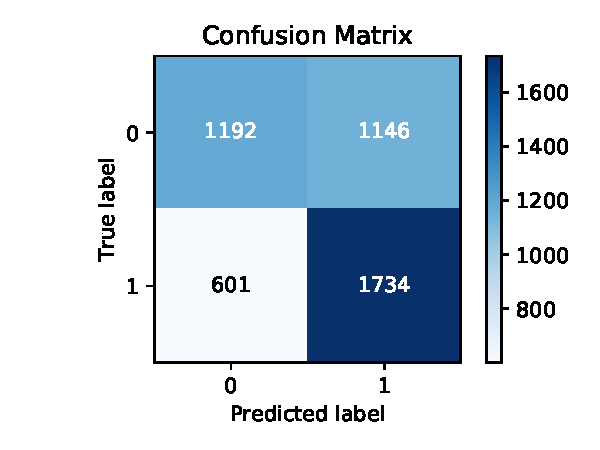
\includegraphics[width=0.4\textwidth, height=0.25\textheight]{figures/logistic_smote_confmat}} 
    \subfloat[Balanced weighting]{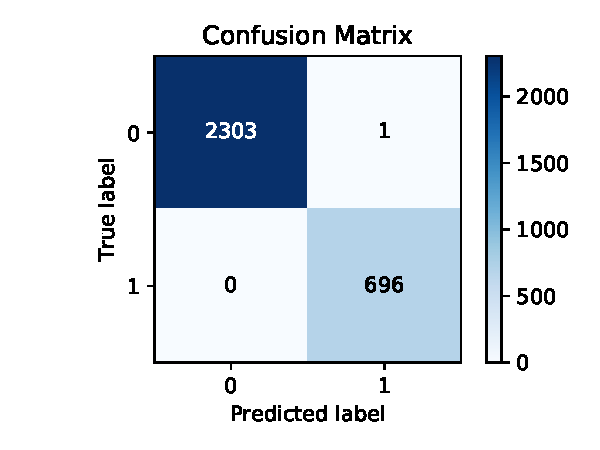
\includegraphics[width=0.4\textwidth, height=0.25\textheight]{figures/logistic_none_balanced_confmat}}
\end{center}
\caption[caption]{Confusion matrices for the logistic regression model using different resampling methods to balance the data set.}
\end{figure}
\begin{figure}[H]\label{fig:logistic3}
\begin{center}
    \subfloat[Random oversampling]{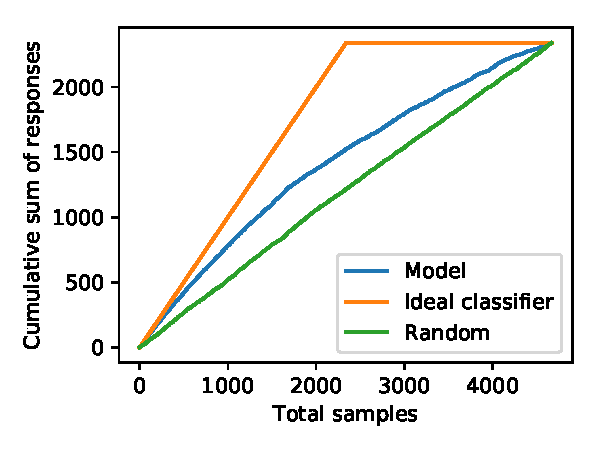
\includegraphics[width=0.4\textwidth, height=0.25\textheight]{figures/logistic_random_oversampling_cumul}} 
    \subfloat[ADASYN]{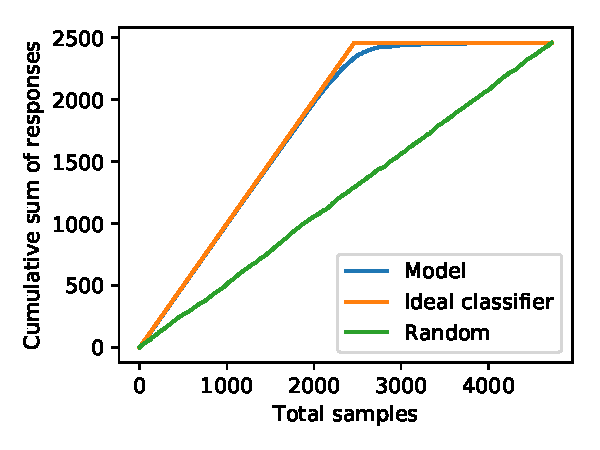
\includegraphics[width=0.4\textwidth, height=0.25\textheight]{figures/logistic_adasyn_cumul}} \\
    \subfloat[SMOTE]{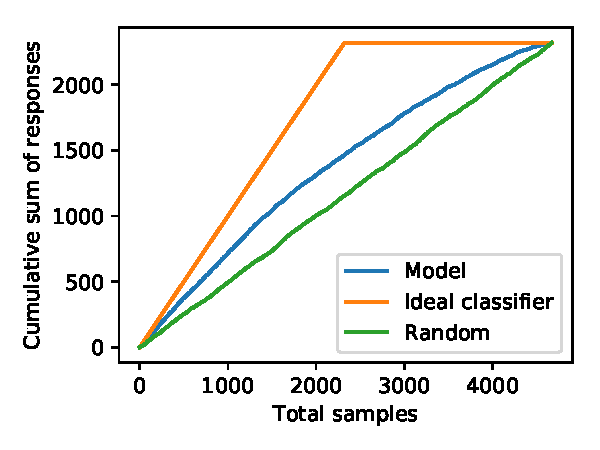
\includegraphics[width=0.4\textwidth, height=0.25\textheight]{figures/logistic_smote_cumul}} 
    \subfloat[Balanced weighting]{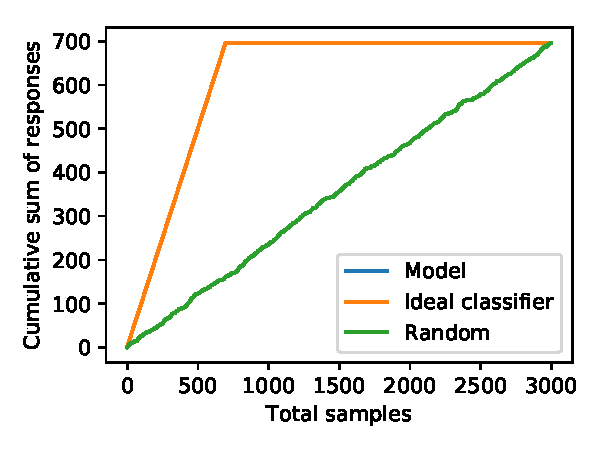
\includegraphics[width=0.4\textwidth, height=0.25\textheight]{figures/logistic_none_balanced_cumul}}
\end{center}
\caption[caption]{Cumulative gain chart for the logistic regression model using different resampling methods to balance the data set.}
\end{figure}
\begin{figure}[H]\label{fig:logistic-roc}
\begin{center}
    \subfloat[Random oversampling]{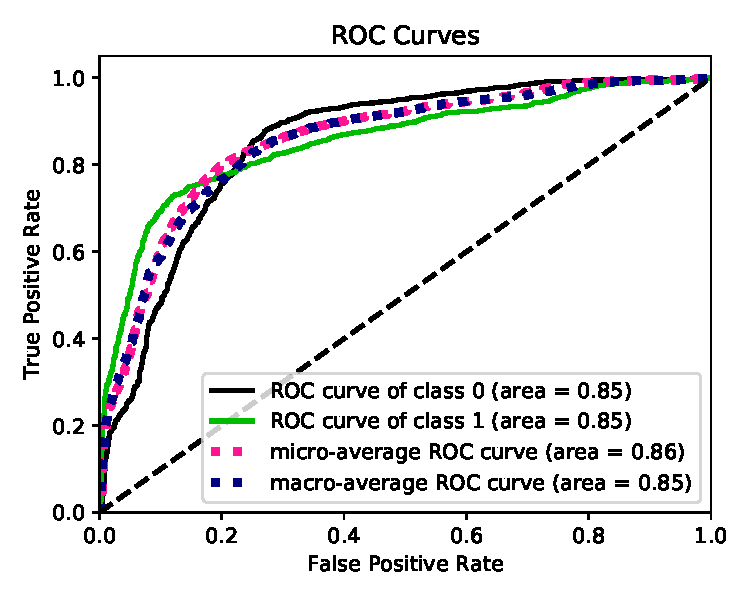
\includegraphics[width=0.4\textwidth, height=0.25\textheight]{figures/logistic_random_oversampling_roc}} 
    \subfloat[ADASYN]{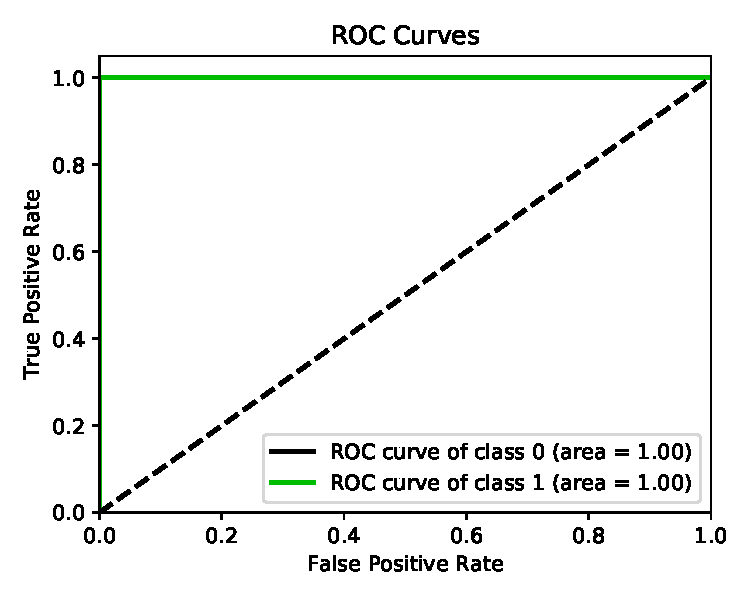
\includegraphics[width=0.4\textwidth, height=0.25\textheight]{figures/logistic_adasyn_roc}} \\
    \subfloat[SMOTE]{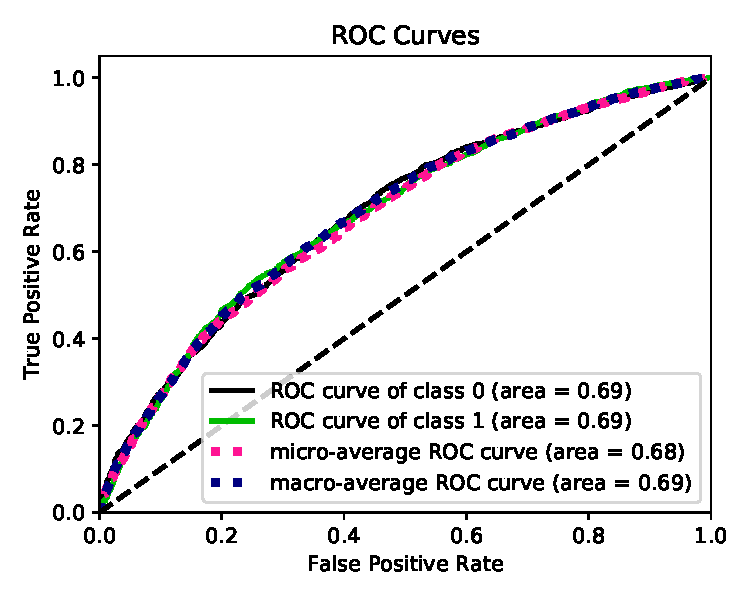
\includegraphics[width=0.4\textwidth, height=0.25\textheight]{figures/logistic_smote_roc}} 
    \subfloat[Balanced weighting]{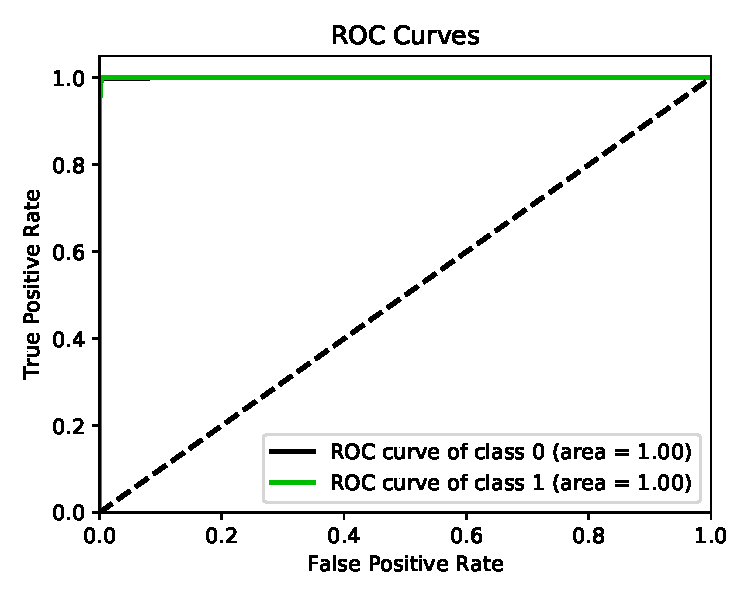
\includegraphics[width=0.4\textwidth, height=0.25\textheight]{figures/logistic_none_balanced_roc}}
\end{center}
\caption[caption]{ROC curves for the logistic regression model using different resampling methods to balance the data set.}
\end{figure}

Results from neural network is included in figure: 
\begin{figure}[H]
\begin{center}
    \subfloat[]{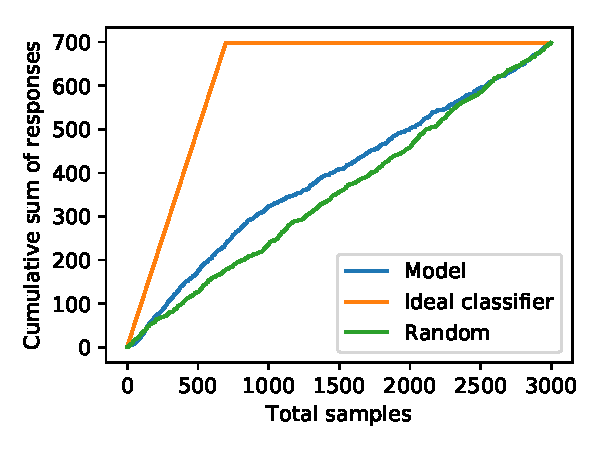
\includegraphics[width=0.4\textwidth, height=0.25\textheight]{figures/net_cumul}} 
    \subfloat[]{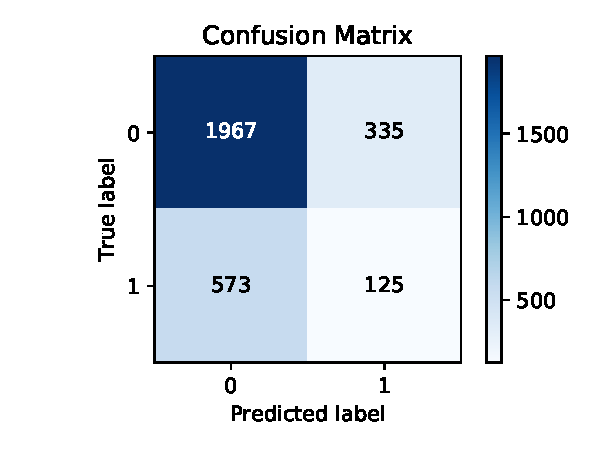
\includegraphics[width=0.4\textwidth, height=0.25\textheight]{figures/net_confmat}} \\
    \subfloat[]{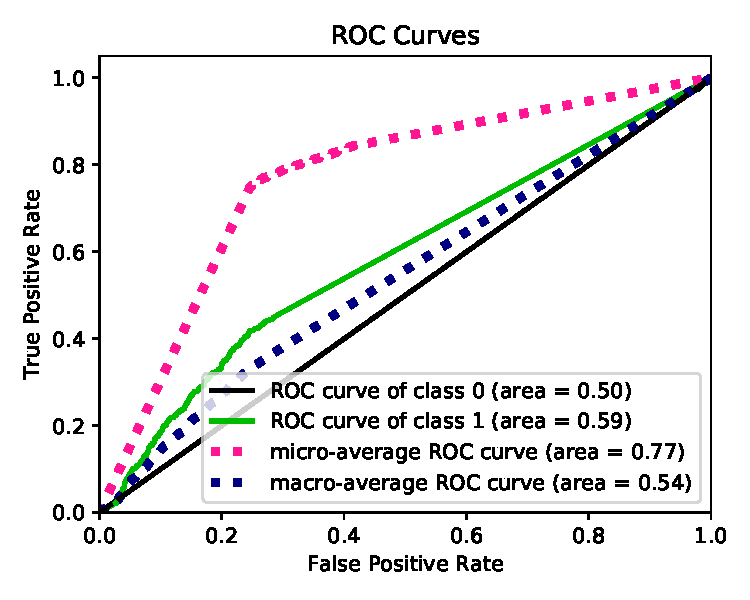
\includegraphics[width=0.5\textwidth]{figures/net_roc}}
\end{center}
\caption[caption]{Performance analysis for neural network classification.}
\end{figure}

Results from random forest is given below
\begin{figure}[H]
\begin{center}
    \subfloat[]{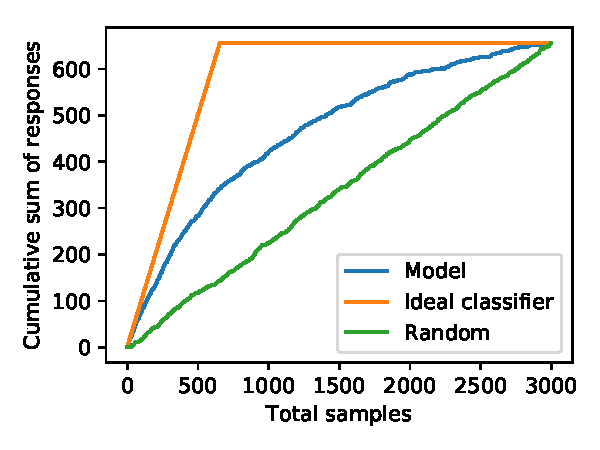
\includegraphics[width=0.4\textwidth, height=0.25\textheight]{figures/forest_cumul}} 
    \subfloat[]{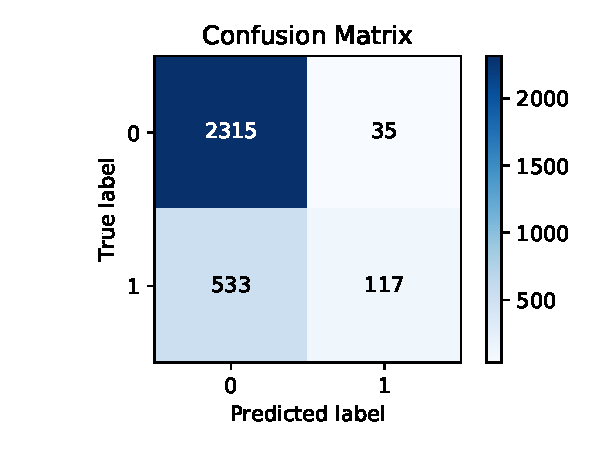
\includegraphics[width=0.4\textwidth, height=0.25\textheight]{figures/forest_confmat}} \\
    \subfloat[]{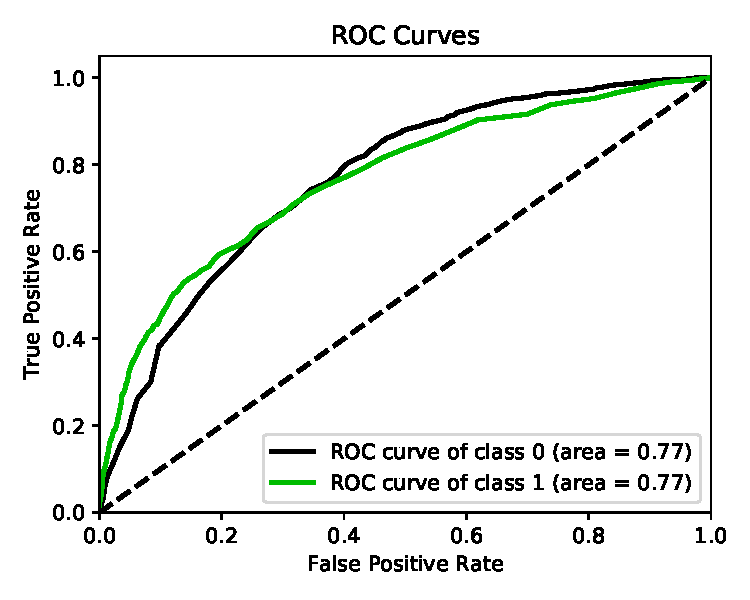
\includegraphics[width=0.5\textwidth]{figures/forest_roc}}
\end{center}
\caption[caption]{Performance analysis for random forest classification.}
\end{figure}


